\newpage
\section{API Documentation}

The API is documented through FastAPI's interactive interface at \url{https://gait-authentication.sigurdurhaukur.com/docs} (or \url{http://localhost:8050/docs} if running locally). The screenshot below shows the endpoint groups and the Pydantic models that define the request and response shapes.

\begin{figure}[H]
    \centering
    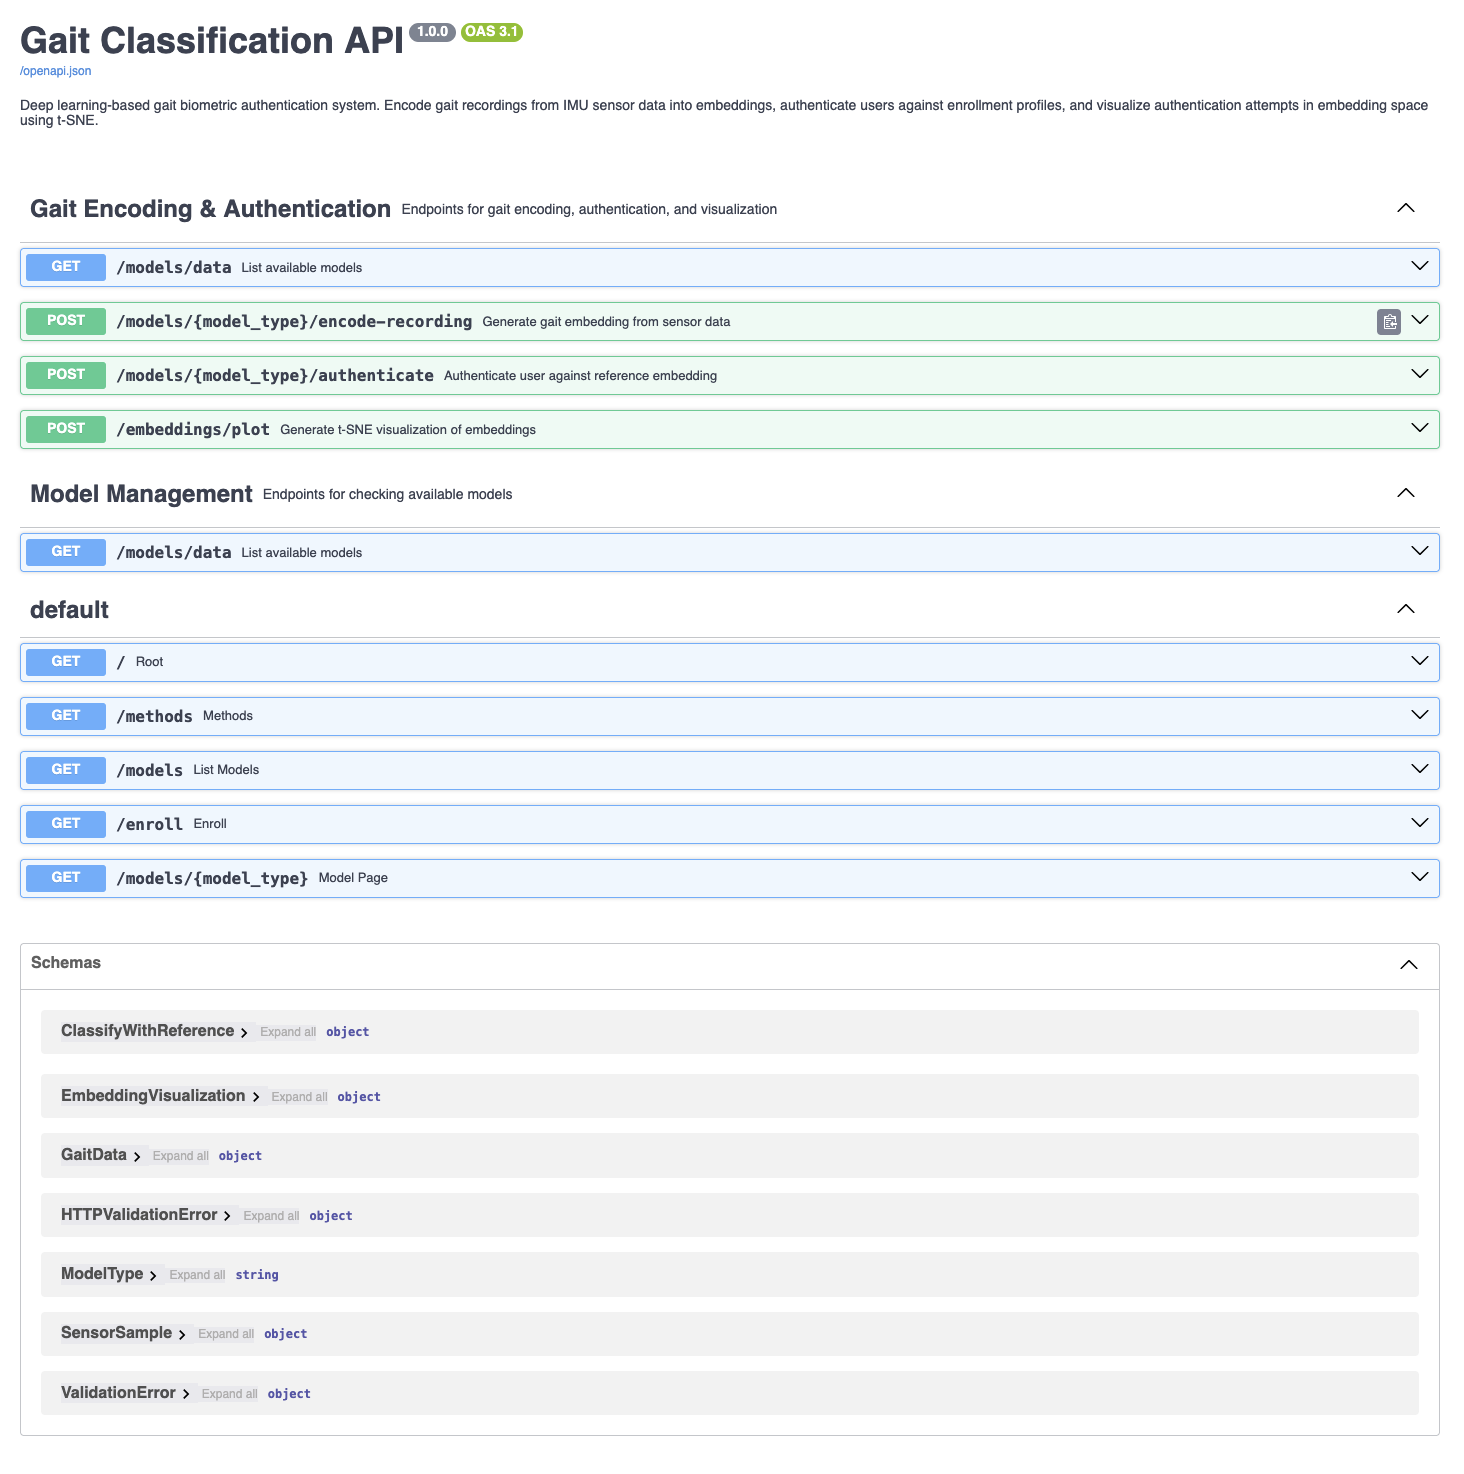
\includegraphics[width=0.98\linewidth]{figures/api-screenshot.png}
    \caption{FastAPI documentation showing the endpoints and schema definitions.}
\end{figure}

The main request types are defined by the following Pydantic models:

\begin{itemize}
    \item \texttt{GaitData}: a list of Inertial Measurement Unit (IMU) sensor samples with accelerometer and gyroscope values.
    \item \texttt{ClassifyWithReference}: gait samples plus a reference embedding for authentication.
    \item \texttt{EmbeddingVisualization}: a reference embedding and authentication history for plotting.
\end{itemize}

The main response endpoints are:

\begin{itemize}
    \item \texttt{/models/\{model\_type\}/encode-recording}: returns an \texttt{embedding} vector.
    \item \texttt{/models/\{model\_type\}/authenticate}: returns a match decision, distance, threshold, confidence, samples processed, and the computed embedding.
    \item \texttt{/embeddings/plot}: returns a t-SNE plot of the reference embedding and authentication history for visualization.
\end{itemize}

The request/response screenshot below shows a successful API call made with \texttt{curl} and the returned JSON response. In this example, we sent IMU data (gyroscope and accelerometer readings) to the \texttt{/models/lstm/encode-recording} endpoint to embedd the gait data, and we received the expected embedding vector in the response, then we sent another request to the \texttt{/models/lstm/authenticate} endpoint with IMU data of a different recording and the previous embedding as a reference (the model compares the similarity of the new embedding with the reference embedding to determine if they match). The response indicates that the two recordings do match, with a distance of 0.4 (just below the threshold of 0.5) and a confidence score of 0.6, meaning the model is reasonably confident that the two recordings are from the same person. The response also includes the number of samples processed and the computed embedding for the new recording. This demonstrates that the API is functioning correctly and can process gait data to perform authentication based on the learned embeddings.

\begin{figure}[H]
    \centering
    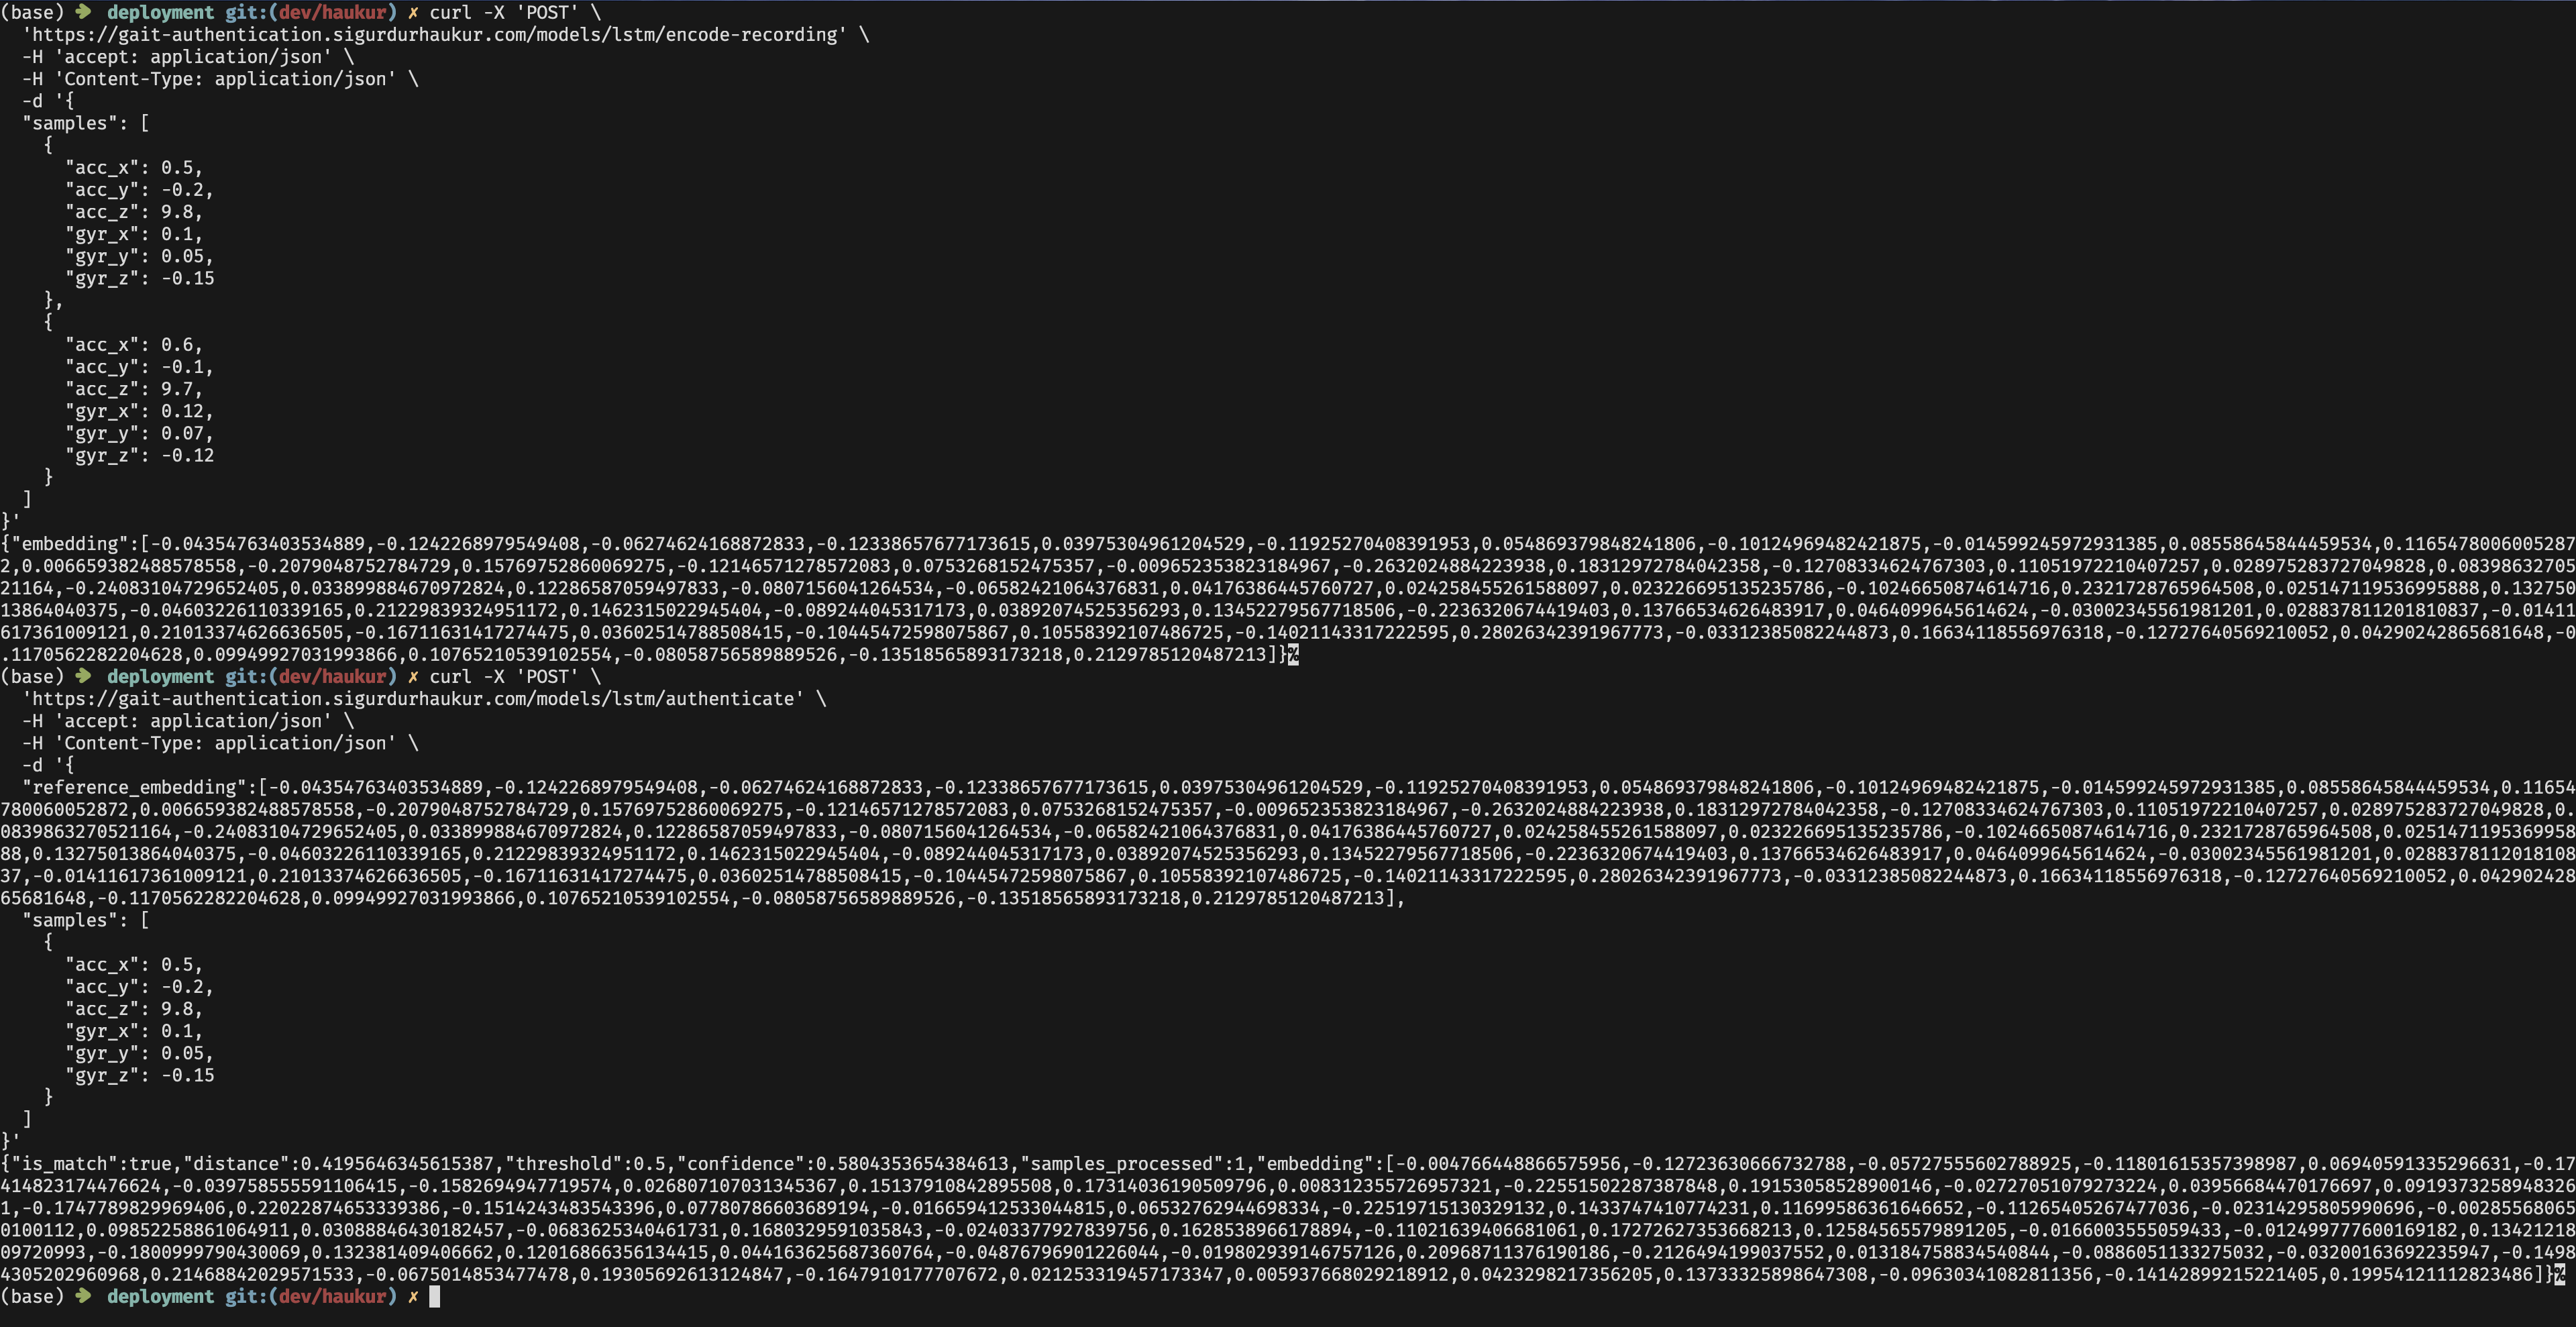
\includegraphics[width=0.98\linewidth]{figures/curl-request-screenshot.png}
    \caption{Example API request and successful response.}
\end{figure}
